\documentclass[letterpaper]{article} % DO NOT CHANGE THIS
\usepackage{aaai27}  % DO NOT CHANGE THIS
\usepackage{times}  % DO NOT CHANGE THIS
\usepackage{helvet}  % DO NOT CHANGE THIS
\usepackage{courier}  % DO NOT CHANGE THIS
\usepackage[hyphens]{url}  % DO NOT CHANGE THIS
\usepackage{graphicx}  % DO NOT CHANGE THIS
\urlstyle{rm}  % DO NOT CHANGE THIS
\def\UrlFont{\rm}  % DO NOT CHANGE THIS
\usepackage{natbib}  % DO NOT CHANGE THIS
\usepackage{caption}  % DO NOT CHANGE THIS
\usepackage{amsmath, amssymb}
\usepackage{booktabs}
\usepackage{multirow}
\usepackage{verbatim}
\frenchspacing  % DO NOT CHANGE THIS
\setlength{\pdfpagewidth}{8.5in}  % DO NOT CHANGE THIS
\setlength{\pdfpageheight}{11in}  % DO NOT CHANGE THIS
\pdfinfo{
/TemplateVersion (2027.1)
/Title (Call Their Bluff: Adaptive Policy Selection in Liar’s Dice)
/Author (Iftach Shoham, Shahar Oded, Gilad Katz)
}
\setcounter{secnumdepth}{0} % May be changed to 1 or 2 if section numbers are desired.

\title{Call Their Bluff: Adaptive Policy Selection in Liar’s Dice}

\author{
Iftach Shoham\textsuperscript{\rm 1}\equalcontrib,
Shahar Oded\textsuperscript{\rm 1}\equalcontrib,
Gilad Katz\textsuperscript{\rm 1}
}
\affiliations{
\textsuperscript{\rm 1}Department of Computer and Information Science, Ben-Gurion University of the Negev\\
\{iftachs, odedshah, giladkz\}@post.bgu.ac.il
}

\begin{document}

\maketitle



\begin{abstract}
Imperfect information games require agents to act under hidden state, stochastic outcomes, and strategic deception. We study opponent adaptation in Liar's Dice, an interpretable domain for sequential bidding and bluffing. Our empirical benchmark compares rule based heuristics, a Bayesian probability model, a Monte Carlo CFR baseline, a population trained Masked PPO policy, and an adaptive policy selection architecture that combines online opponent type inference with a portfolio of PPO response policies. The adaptive agent improves performance to 97.8\% across 5,800 matches in a closed-set evaluation over recurring reference opponent types, despite imperfect online identification. Rather than proposing a general game solver, our results show when type conditioned policy reuse can improve over fixed policies in a controlled multiagent setting.
\end{abstract}




\section{Introduction}

Liar’s Dice is a compact imperfect information game in which agents make sequential decisions under private information, stochastic outcomes, and strategic deception. Each player observes only their own dice and must reason about both the hidden dice of others and the behavioral tendencies that shape future bids and challenges. These properties make Liar’s Dice a useful benchmark for studying adaptive decision making in multiagent systems: it is small enough to support controlled experimentation, yet rich enough to expose the limits of fixed strategies under opponent heterogeneity.

The central question in this paper is how agents should trade off worst case robustness against opponent specific exploitation. Much prior work on imperfect information games emphasizes strategies that approximate Nash equilibrium or equilibrium-like behavior, using methods such as Counterfactual Regret Minimization (CFR)~\cite{cfr} or reinforcement learning with self-play and abstraction~\cite{heinrich2016deep}. Such approaches are valuable because they seek policies that are difficult to exploit. However, in practical multiagent environments, opponents are rarely worst case optimizers: they often follow systematic heuristics, exhibit biased risk preferences, or repeat recognizable bluffing patterns. In these cases, a policy that can infer and exploit opponent regularities may outperform a single globally robust policy.

In this work, adaptation is studied in a closed-set sense: the agent is evaluated against recurring opponent types represented in an offline policy library, rather than against arbitrary unseen strategic agents. This setting allows us to isolate whether opponent-type inference and specialist policy reuse can improve empirical performance when opponents exhibit stable behavioral structure.


We investigate this trade-off through a systematic empirical study of Liar’s Dice agents. Our evaluation compares hand-crafted heuristics, a Bayesian probability model, an approximate game-theoretic MCCFR policy, a population trained PPO generalist, and an adaptive agent that performs online opponent type inference and selects from a portfolio of opponent specific response policies. Rather than presenting Liar’s Dice only as a game solving problem, we frame it as a controlled testbed for opponent modeling, policy reuse, and adaptation under partial observability.

Our contributions are as follows:
\begin{itemize}

\item \textbf{Adaptive policy selection architecture:} We evaluate a modular adaptive agent that performs online opponent type inference and selects from opponent specific Masked-PPO response policies trained offline. The goal is not to learn a universal game solving policy, but to test whether type conditioned policy reuse improves performance when opponents exhibit recurring behavioral structure.


\item \textbf{Empirical benchmark study:} We implement and compare a diverse set of Liar's Dice agents, including heuristic policies, a likelihood-based Bayesian agent, an approximate MCCFR policy, and a population trained PPO generalist. This tournament provides a controlled empirical benchmark for studying robustness and exploitation under imperfect information.


\item \textbf{Behavioral and generalization insights:} We analyze how fixed and adaptive policies differ in bidding, challenge behavior, positional effects, latency, and multiagent transfer. The results show that the PPO generalist reaches a 93.14\% win rate among fixed agents, the Bayesian baseline reaches 92.36\%, and the adaptive architecture reaches 97.8\% across the full evaluation pool despite imperfect online identification.
\end{itemize}
Our results show that fixed policies can be highly effective but remain locally exploitable against particular opponents and player roles. The adaptive agent helps close this gap by using opponent identity as an explicit decision variable. This finding supports a workshop-relevant perspective on multiagent learning: empirical strength in realistic strategic settings may require not only equilibrium-inspired robustness, but also mechanisms for recognizing and reusing specialized responses to recurring opponent behaviors.


\section{Preliminaries and Problem Setting}
Liar's Dice is an imperfect information game with private dice, sequential public bids, and challenge actions. A bid states that at least a given quantity of dice across all players show a chosen face; subsequent bids must strictly increase the claim, and a challenge reveals all dice and resolves the round. This structure exposes three properties central to adaptive multiagent learning: hidden state, stochastic outcomes, and opponent dependent deception. We focus primarily on full two player matches with five dice per player, while retaining a small multiagent transfer study to probe whether learned representations scale beyond the training setting.

We evaluate agents under the same information constraints available to a human player: private dice, public dice counts, the current bid, and public action history. The main empirical question is not whether Liar's Dice can be solved in general, but whether opponent-conditioned policy reuse improves over fixed policies when opponents exhibit recurring behavioral structure. Detailed game rules, heuristic-agent definitions, and MCCFR implementation details are provided in the supplementary material.


\section{Methodology}
\subsection{Agent Population}
We implement a diverse evaluation population spanning rule based heuristics, probability-driven play, approximate equilibrium play, and learned policies. Heuristic agents cover conservative and aggressive bidding, minimum- and maximum-raise preferences, frequency based openings, threshold challenge rules, stochastic bidding, and deliberately irregular behaviors. The Bayesian agent evaluates each bid using a binomial likelihood over unobserved dice and challenges when the estimated probability of truth falls below a turn dependent threshold. The MCCFR agent is trained offline with simplified information sets and serves as an approximate game-theoretic baseline rather than a fully converged equilibrium policy.

The population trained RL baseline is a Masked-PPO policy. The action mask removes illegal bids and unavailable challenges, while the observation encodes private face counts, remaining dice, the current bid, and a short window of recent actions. Training uses a two-stage curriculum: first against fixed opponents of increasing complexity, then against a league sampled with loss weighted opponent probabilities. The resulting PPO policy is frozen at evaluation time and receives no explicit opponent identity.

\subsection{Adaptive Policy-Selection Agent}
The main contribution is a modular adaptive agent that separates \emph{opponent inference} from \emph{response execution}. It maintains a belief over a finite set of reference opponent types, each corresponding to one policy in the evaluation population. A neural sequence classifier processes the observed action trajectory and outputs a distribution over opponent types. Predictions are smoothed over time to avoid unstable policy switching.

Conditioned on the most likely opponent type, the adaptive agent selects a pre-trained Masked-PPO response policy from a portfolio of specialists. Each specialist is trained offline against one reference opponent and then frozen. At test time, no gradient updates, regret updates, or online planning are performed; adaptivity comes only from updating the inferred opponent type and switching the selected response policy. This design intentionally tests a limited but practical form of adaptation: whether type conditioned policy reuse can exploit recurring opponent structure without claiming general open set game solving.

\begin{figure*}[t]
    \centering
    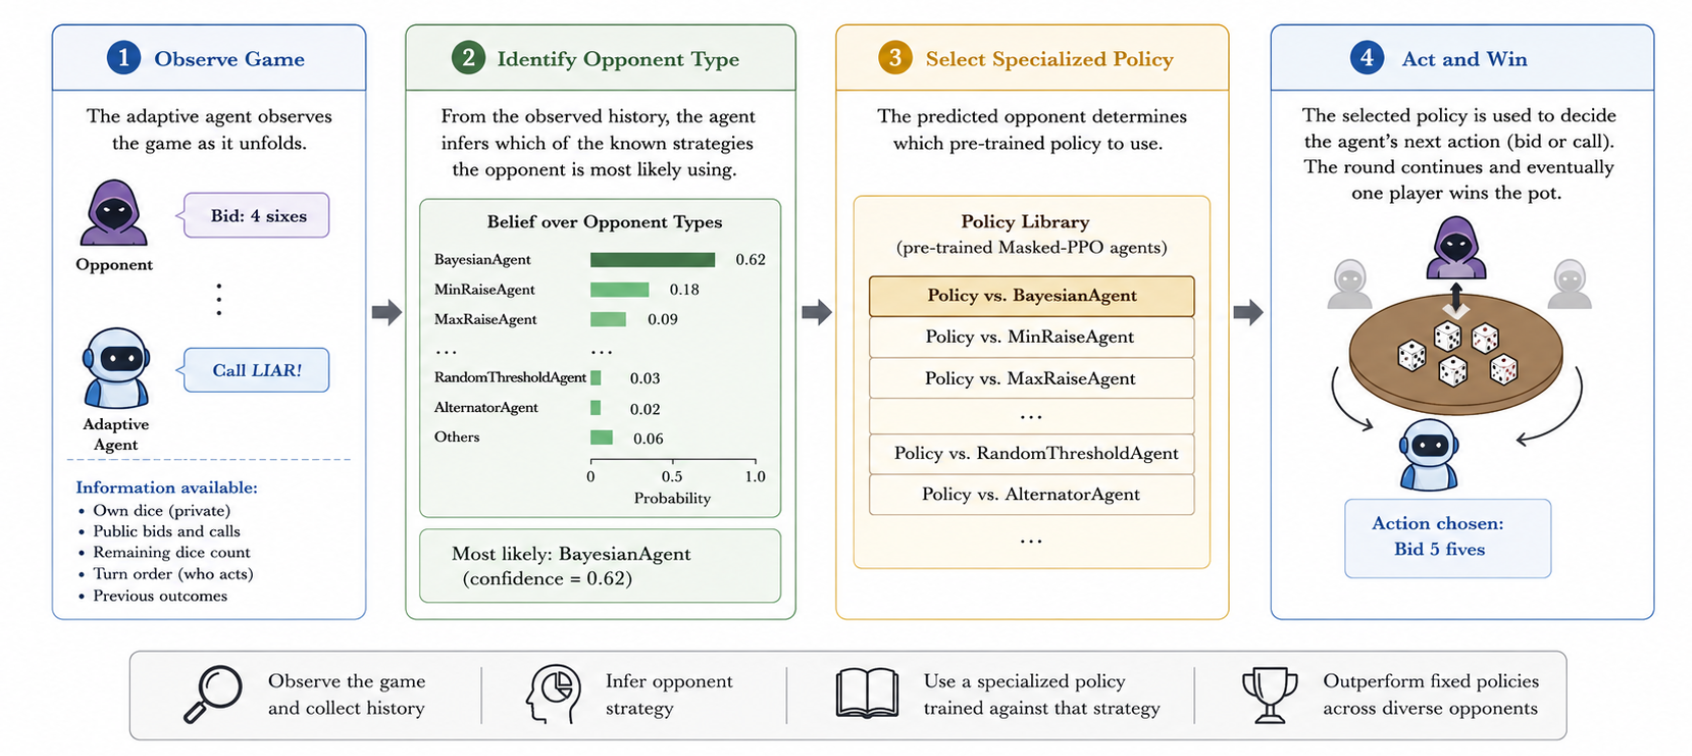
\includegraphics[width=0.98\textwidth]{images/overview.png}
    \caption{Overview of the adaptive agent. 
    At each decision point, the agent (1) observes the game state and history, (2) infers the opponent's strategy among a set of known types, (3) selects the corresponding pre-trained policy optimized against that type, and (4) acts according to this policy to maximize the probability of winning the match.}
    \label{fig:adaptive_agent_overview}
\end{figure*}

\section{Experimental Setup}
All agents play full matches until one player loses all dice. The fixed-policy tournament uses 200 games per ordered agent pairing, giving 400 games across both role assignments for each distinct pair. Other evaluations use the sample sizes stated in their respective sections. We report aggregate win rate, position conditioned win rate, opponent identification accuracy, and qualitative behavioral statistics. Learning-based agents are trained offline and frozen during evaluation. PPO uses a learning rate of $3\times 10^{-4}$, discount factor $\gamma=0.99$, batch size 128, and entropy coefficient 0.05. The generalist PPO is trained for approximately $1.15$M environment steps; each adaptive response policy is trained for up to $500{,}000$ steps against its reference opponent. The opponent classifier is trained for 50 epochs on trajectories collected from baseline-agent play and reaches 83.9\% validation accuracy.

\section{Results}
\subsection{Fixed-Policy Benchmark}
Table~\ref{tab:fixed_benchmark} summarizes the strongest fixed agents.
The PPO generalist obtains the best aggregate win rate among fixed policies, closely followed by the Bayesian agent. The approximate MCCFR baseline remains near parity, reflecting the limitations of simplified information sets and bounded training rather than a definitive weakness of regret minimization. The supplementary material reports the full fixed-agent tournament table and the role-conditioned head-to-head matrix. These results motivate adaptation: fixed policies can be strong on average while retaining localized weaknesses against specific opponent types and player positions.

\begin{table}[t]
\centering
\small
\begin{tabular}{lccc}
\toprule
Agent & Win \% & P0 Win \% & P1 Win \% \\
\midrule
PPO generalist & \textbf{93.14} & 90.54 & \textbf{95.73} \\
Bayesian       & 92.36 & \textbf{95.63} & 89.10 \\
MCCFR          & 45.42 & 45.12 & 45.71 \\
\bottomrule
\end{tabular}
\caption{Condensed fixed-policy benchmark. PPO is the strongest fixed policy overall, while role-conditioned results show that fixed strategies remain position-sensitive.}
\label{tab:fixed_benchmark}
\end{table}

Policy diagnostics explain this pattern. MCCFR exhibits sharp, quantity-driven challenge thresholds and concentrated opening bids, while PPO learns smoother call-liar behavior and more diverse openings. The supplementary material includes the omitted call-liar heatmaps and opening-bid distributions. The Bayesian agent is competitive because the bid-truth likelihood is highly informative in this domain. However, no fixed policy dominates every matchup: PPO is near parity against the Bayesian and Alternator agents, suggesting that population-level strength and targeted exploitability coexist.

\subsection{Adaptive-Agent Performance}
The adaptive agent achieves a 97.8\% aggregate win rate over 5{,}800 matches, with 97.1\% as the first player and 98.4\% as the second player. This improves over the strongest fixed policy and substantially reduces positional asymmetry. Importantly, this gain does not require perfect online identification. Although the classifier reaches 83.9\% offline validation accuracy, online identification over partial trajectories is 48.81\% under a strict exact-type definition. Low exact type accuracy does not necessarily imply poor response selection, because several reference opponents induce similar strategic responses. Thus, the selected specialist may be behaviorally appropriate even when the nominal opponent label is incorrect. When identification succeeds, it occurs quickly: the mean time to correct identification is $2.76 \pm 0.92$ decision steps, with median 2.


\begin{table}[t]
\centering
\small
\begin{tabular}{@{}lccc@{}}
\toprule
Slice & Win \% & ID Acc. & Steps \\
\midrule
All & \textbf{97.8} & 48.81 & $2.76\pm0.92$ \\
Structured & 99--100 & 69.5--100 & 2.0--3.4 \\
Stochastic/weak & 90--100 & 0--50 & 2.0--4.0 \\
Alternator & 53.0 & 26.5 & 2.0 \\
\bottomrule
\end{tabular}
\caption{Adaptive-agent performance. Type-conditioned response selection improves aggregate win rate despite imperfect online identification, but Alternator remains a difficult non-informative stress test.}
\label{tab:adaptive_summary}
\end{table}

Table~\ref{tab:adaptive_summary} highlights both the strength and the limitation of the adaptive architecture. The agent reaches perfect or near perfect win rates against most structured heuristic, Bayesian, PPO, and MCCFR opponents. The supplementary material reports per-opponent identification accuracy, identification speed, and role-conditioned win rates for every evaluated opponent. Against stochastic or overlapping strategies, exact type identification becomes less reliable, but the selected response policies often remain competitive because nearby experts provide useful coverage. The main failure case is Alternator, which deterministically alternates between challenges and minimum raises and therefore provides little stable strategic signal to exploit. The adaptive agent wins only 53\% in this matchup, underscoring that the method is not a general solution for arbitrary unseen or intentionally non-informative opponents.

\subsection{Evaluation Against LLM-Based Opponents}

We additionally evaluate the adaptive agent against three LLM-based opponents from OpenAI:
\texttt{gpt-4o-mini},\linebreak \texttt{gpt-4.1-mini}, and \texttt{gpt-5.4-nano}. This serves as an out-of-distribution stress test, since these opponents were not included in the reference set used for opponent classification or specialist policy training. Each matchup consists of 50 full games, split evenly across player positions.

\begin{table}[t]
\centering
\small
\begin{tabular}{lccc}
\hline
Opponent  & Win \% & P0 Win \% & P1 Win \%  \\
\hline
\texttt{gpt-4o-mini}   & 52.0  & 56.0 & 48.0   \\
\texttt{gpt-4.1-mini}  & 94.0  & 100.0 & 88.0 \\
\texttt{gpt-5.4-nano}  & 94.0 & 92.0 & 96.0   \\
\hline
\end{tabular}
\caption{
Adaptive-agent performance against LLM-based opponents. Win rate is reported
from the adaptive agent's perspective. P0 and P1 denote the adaptive agent's
player position.
}
\label{tab:llm_opponents}
\end{table}

The adaptive agent is near parity against \texttt{gpt-4o-mini}, but wins
94.0\% of games against both \texttt{gpt-4.1-mini} and \texttt{gpt-5.4-nano}.





\section{Additional Analysis}
Latency remains low enough for interactive play. Rule-based, Bayesian, and MCCFR agents act in under $0.02$ ms on average, while PPO and adaptive agents require roughly $0.57$ ms and $0.74$ ms per decision, respectively. Multi-agent transfer reveals a representation limitation: the PPO policy was trained with a two player observation encoding and collapses when deployed zero shot to three or four player games, whereas the Bayesian agent naturally scales its binomial model with the number of dice. The supplementary material includes the latency table, behavioral-correlation matrix, and multi-agent transfer table. This supports our broader benchmark insight: learned policies can be highly effective in distribution, but scalable adaptation requires state representations that match the deployment setting.



\section{Related Work}
Prior work on imperfect information games often emphasizes equilibrium oriented robustness. Counterfactual Regret Minimization and Monte Carlo variants minimize regret over information sets and have been used in poker-like games and Liar's Dice-style domains \cite{cfr,mccfr}. Deep CFR, NFSP, and ReBeL extend this line with function approximation, self-play, and search \cite{brown2019deep,heinrich2016deep,kawamura2017neural,brown2020combining}. These methods provide strong game-theoretic motivation, but their focus on equilibrium play can leave performance gains unused against systematic non-equilibrium opponents.

Our work instead aligns with opponent modeling, policy reuse, and population-based learning. Opponent-aware agents can infer behavioral regularities from interaction and adapt their responses \cite{he2016opponent,yu2022model,jing2024opponent,yu2024opponent}. PSRO and Bayesian policy reuse similarly motivate maintaining a population or library of policies and selecting responses based on opponent characteristics \cite{lanctot2017unified,rosman2016bayesian}. We contribute a compact empirical study in Liar's Dice that compares fixed probabilistic, regret-minimization, and learned policies against a type conditioned adaptive architecture.


\section{Limitations}
Our evaluation is empirical and population-based. It should not be interpreted as a formal exploitability analysis or as evidence that type conditioned policy reuse generalizes to arbitrary unseen opponents. Training cost is also not normalized across methods: heuristics require no training, MCCFR uses offline regret minimization with simplified information sets, and PPO-based methods require substantial simulation. Finally, the adaptive agent assumes a finite reference set of opponent types; open set recognition and uncertainty aware policy blending remain necessary for deployment against truly novel behaviors.



\section{Conclusion}
We presented a dense empirical study of adaptive decision-making in Liar's Dice, centered on a modular opponent-type inference and policy selection architecture. The benchmark shows that a population trained PPO policy and a simple Bayesian agent are strong fixed baselines, but that fixed policies remain locally exploitable. The adaptive agent improves aggregate performance by selecting among frozen opponent specific PPO response policies, achieving 97.8\% win rate across the evaluated population despite imperfect online identification. The central takeaway is not a new general game solver, but a workshop-relevant benchmark insight: in repeated imperfect information interactions, recognizing recurring opponent structure can make policy reuse substantially more effective than committing to a single fixed policy.

\section{Future Work}
Future work should extend this framework to open set opponent recognition, uncertainty aware mixtures of response policies, and multiagent observation encodings that scale beyond two player play. Another important direction is safe exploitation: adapting to opponent regularities while bounding worst case vulnerability when the inferred type is wrong.

\clearpage
\bibliographystyle{aaai27}

% Loading bibliography database
\bibliography{bib}

\clearpage
\section*{Supplementary Material}
\appendix

\subsection{Liar’s Dice Rules and Game Mechanics}
\label{app:rules}

In the game, each player holds a private set of dice, while the dice of other players remain hidden. Game play consists of sequential bidding and challenges, with players reasoning probabilistically about unknown outcomes and strategically interpreting opponent actions.

\paragraph{\textbf{Players and Dice}}

The game consists of $N$ players. At the start of each round, each player is assigned $D$ fair six-sided dice, which are rolled privately. A player’s dice constitute their private information; the total number of dice in play is $N \times D$.

\paragraph{\textbf{Bidding Actions}}

Players take turns in a fixed order. On their turn, a player must either place a bid or challenge the most recent bid. A bid is an assertion $(q, f)$, where: $q \in N \times D$ is a quantity, $f \in \{1,2,3,4,5,6\}$ is a face value. The bid $(q, f)$ claims that among all dice in play, at least $q$ dice show face value $f$.

Bids must strictly increase according to a predefined ordering, prioritizing higher quantities and, secondarily, higher face values.

\paragraph{\textbf{Challenge Action}}

Instead of bidding higher, a player may challenge the most recent bid. When a bid $(q, f)$ is challenged, all dice from all players are revealed. If at least $q$ dice shows the face value $f$, the bid is valid; otherwise, it is invalid.

\paragraph{\textbf{Round Resolution and Payoffs}}

If the bid is valid, the challenger loses the round; if invalid, the bidder loses. The losing player forfeits one die, and a new round begins with all remaining dice re-rolled privately. The winner of the last round will be the first to bid in the next round.

\paragraph{\textbf{Game Termination}}

The game continues until only one player remains with at least one die. Since at most one die is lost per round and eliminating \(N-1\) players requires removing \(D\) dice from each, the game length is bounded below by \(D (N-1)\) rounds.

\paragraph{\textbf{Imperfect Information and Strategic Considerations}}

Because players observe only their own dice, Liar’s Dice requires reasoning over hidden information and opponent behavior. Bids convey both probabilistic claims and strategic intent, serving not only as stochastic signals about the game state but also as indicators of a player’s broader strategy.



\subsection{\textbf{Heuristic Agents}}
\label{app:heuristic_agents}

We implement a family of \emph{heuristic agents} that rely on simple, rule-based decision policies rather than explicit probabilistic inference. These agents serve as interpretable baselines and are designed to span a diverse space of bidding and challenge behaviors, isolating strategic dimensions such as risk tolerance, raise magnitude, belief approximation, and stochasticity.

\paragraph{\textbf{Common structure}}
All heuristic agents operate on the same observable information: the agent’s private dice, the current public bid, and the total number of dice in play. A bid \( b = (q,f) \) is treated as \emph{impossible} if its quantity exceeds the total number of dice; such bids are always challenged. Otherwise, agents choose between calling liar and producing a higher legal bid according to fixed rules.

\paragraph{\textbf{Conservative and aggressive bidding}}
At one extreme, the \emph{Conservative} agent challenges aggressively, calling liar whenever bids grow large and otherwise making minimal raises. At the other extreme, the \emph{Aggressive} agent prefers to continue bidding whenever possible, typically raising quantities and only calling liar when no legal raise remains. These agents model risk-averse and risk-seeking behaviors, respectively.

\paragraph{\textbf{Raise-preference heuristics}}
Several agents differ only in how they select among legal raises. \emph{Minimal-raise} agents always choose the smallest valid increase, while \emph{maximal-raise} agents choose the largest. These policies isolate the strategic effect of cautious versus forceful bidding without additional belief modeling.

\paragraph{\textbf{Frequency-based heuristics}}
Some agents exploit simple statistics of their private dice. For example, the \emph{MaxCount} agent opens by bidding the face it holds most frequently, while \emph{SafeFace} agents prefer bidding faces already present in hand. Variants such as \emph{Ones-Are-Wild} explicitly bias bids toward face \(1\) when wild-card rules apply.

\paragraph{\textbf{Threshold and expectation heuristics}}
Threshold-based agents call liar whenever the bid quantity exceeds a fixed or randomly chosen cutoff (e.g., half the total dice). The \emph{Probability} agent uses a crude expectation heuristic, comparing the bid quantity to the expected count \( D / |\mathcal{F}| \), where \( \mathcal{F} \) is the set of faces, without computing exact probabilities.

\paragraph{\textbf{Stochastic and adversarial behaviors}}
To increase behavioral diversity, we include agents that introduce randomness or non-standard logic, such as \emph{Bluffing} agents (occasionally bidding faces not in hand), \emph{Chaotic} agents (randomly choosing between raising and challenging), and pattern-based agents (e.g., parity- or cycle-based bidding).


\subsection{Approximate Nash Agent (Monte Carlo CFR)}
\label{app:mccfr_agent}

To approximate equilibrium play, we implement a Nash-style agent based on \emph{External Sampling Monte Carlo Counterfactual Regret Minimization} (MCCFR)\cite{mccfr}. This agent represents a game-theoretic baseline beyond heuristic or myopic strategies, as it approximates a Nash equilibrium in extensive-form games.

\paragraph{\textbf{Game model and information sets}}
The agent models Liar’s Dice as an extensive-form game with imperfect information. An information set is defined as
\[
I = (d_{\text{me}}, q_{\text{last}}, f_{\text{last}}),
\]
where \( d_{\text{me}} \) denotes the agent’s private dice (sorted), and \( (q_{\text{last}}, f_{\text{last}}) \) denotes the most recent public bid (or \texttt{None} at the start of the game). The agent does not observe opponent dice, only their aggregate count.

\paragraph{Policy representation.}
For each dice configuration and face set, the learned strategy is stored as a policy
\[
\pi_I(a) \in [0,1],
\quad \sum_{a \in A(I)} \pi_I(a) = 1,
\]
where \( A(I) \) is the set of legal actions at information set \( I \), consisting of all valid higher bids and the action \texttt{call\_liar}. At inference time, actions are sampled according to the learned distribution \( \pi_I \).

\paragraph{\textbf{Training via MCCFR}}
Training is performed offline using external-sampling MCCFR. At each iteration:
\begin{enumerate}
    \item Dice outcomes for all players are sampled (chance sampling).
    \item One player is designated as the traversing player.
    \item For traversing nodes, all actions are explored to update counterfactual regrets.
    \item For opponent nodes, a single action is sampled according to the current strategy.
\end{enumerate}

Regret matching is used to derive strategies from cumulative regrets. Let
\[
Z_I = \sum_{a'} \max(R_I(a'), 0).
\]
Then
\[
\pi_I(a) =
\begin{cases}
\dfrac{\max(R_I(a), 0)}{Z_I}, & \text{if } Z_I > 0, \\ \\
\dfrac{1}{|A(I)|}, & \text{otherwise}.
\end{cases}
\]

\paragraph{\textbf{Utility definition}}
Terminal utilities are assigned only when a \texttt{call\_liar} action occurs. Let \( b = (q,f) \) be the last bid. If the bid is true, the caller receives utility \(-1\); otherwise, the caller receives \(+1\). Utilities are zero-sum between players.

\paragraph{\textbf{Convergence monitoring}}
Optionally, the algorithm tracks convergence by measuring the maximum change in strategy probabilities across sampled information sets. Training halts early if this change falls below a predefined threshold.

\paragraph{\textbf{Deployment and fallback policy}}
At runtime, the agent loads pre-trained policies indexed by dice-count configurations. If no matching policy is found, the agent \textbf{fallback} to selecting a random legal action. This agent is limited to our game configurations, as changes in maximal dice count, players or rules may expose new states the agent was not trained on and skew regrets.

\paragraph{\textbf{Training configuration}}
The MCCFR agent is trained offline using external-sampling Monte Carlo CFR for a fixed dice configuration. Training proceeds for a maximum of $10{,}000$ iterations, unless early convergence is detected. At each iteration, a full chance sample of player dice is drawn, and two traversal passes are executed, one for each player as the traversing player.

Optionally, convergence is monitored by tracking changes in the agent’s average strategy. Every $500$ iterations, the normalized action probabilities derived from the accumulated strategy sums are compared against a stored snapshot from the previous checkpoint. Convergence is declared when the maximum absolute change in action probability across a sampled subset of information sets falls below a threshold of $0.001$, at which point training terminates early.

This criterion reflects empirical stabilization of the learned policy rather than formal exploitability bounds, and is used to prevent unnecessary additional sampling once the strategy distribution ceases to change meaningfully.
\subsection{Supplementary Result Tables and Figures}
\label{app:supplementary_results}

This section preserves the detailed result material omitted from the compact workshop submission. The main paper reports condensed summaries; the tables and figures here provide the fuller diagnostics used to support those summaries.

\paragraph{Policy-level PPO--MCCFR comparisons.}
Figures~\ref{fig:app_mccfr_call_liar}--\ref{fig:app_mccfr_opening} report the call-liar and opening-bid distributions used to compare the population-trained PPO policy against the MCCFR baseline.

\begin{figure}[t]
    \centering
    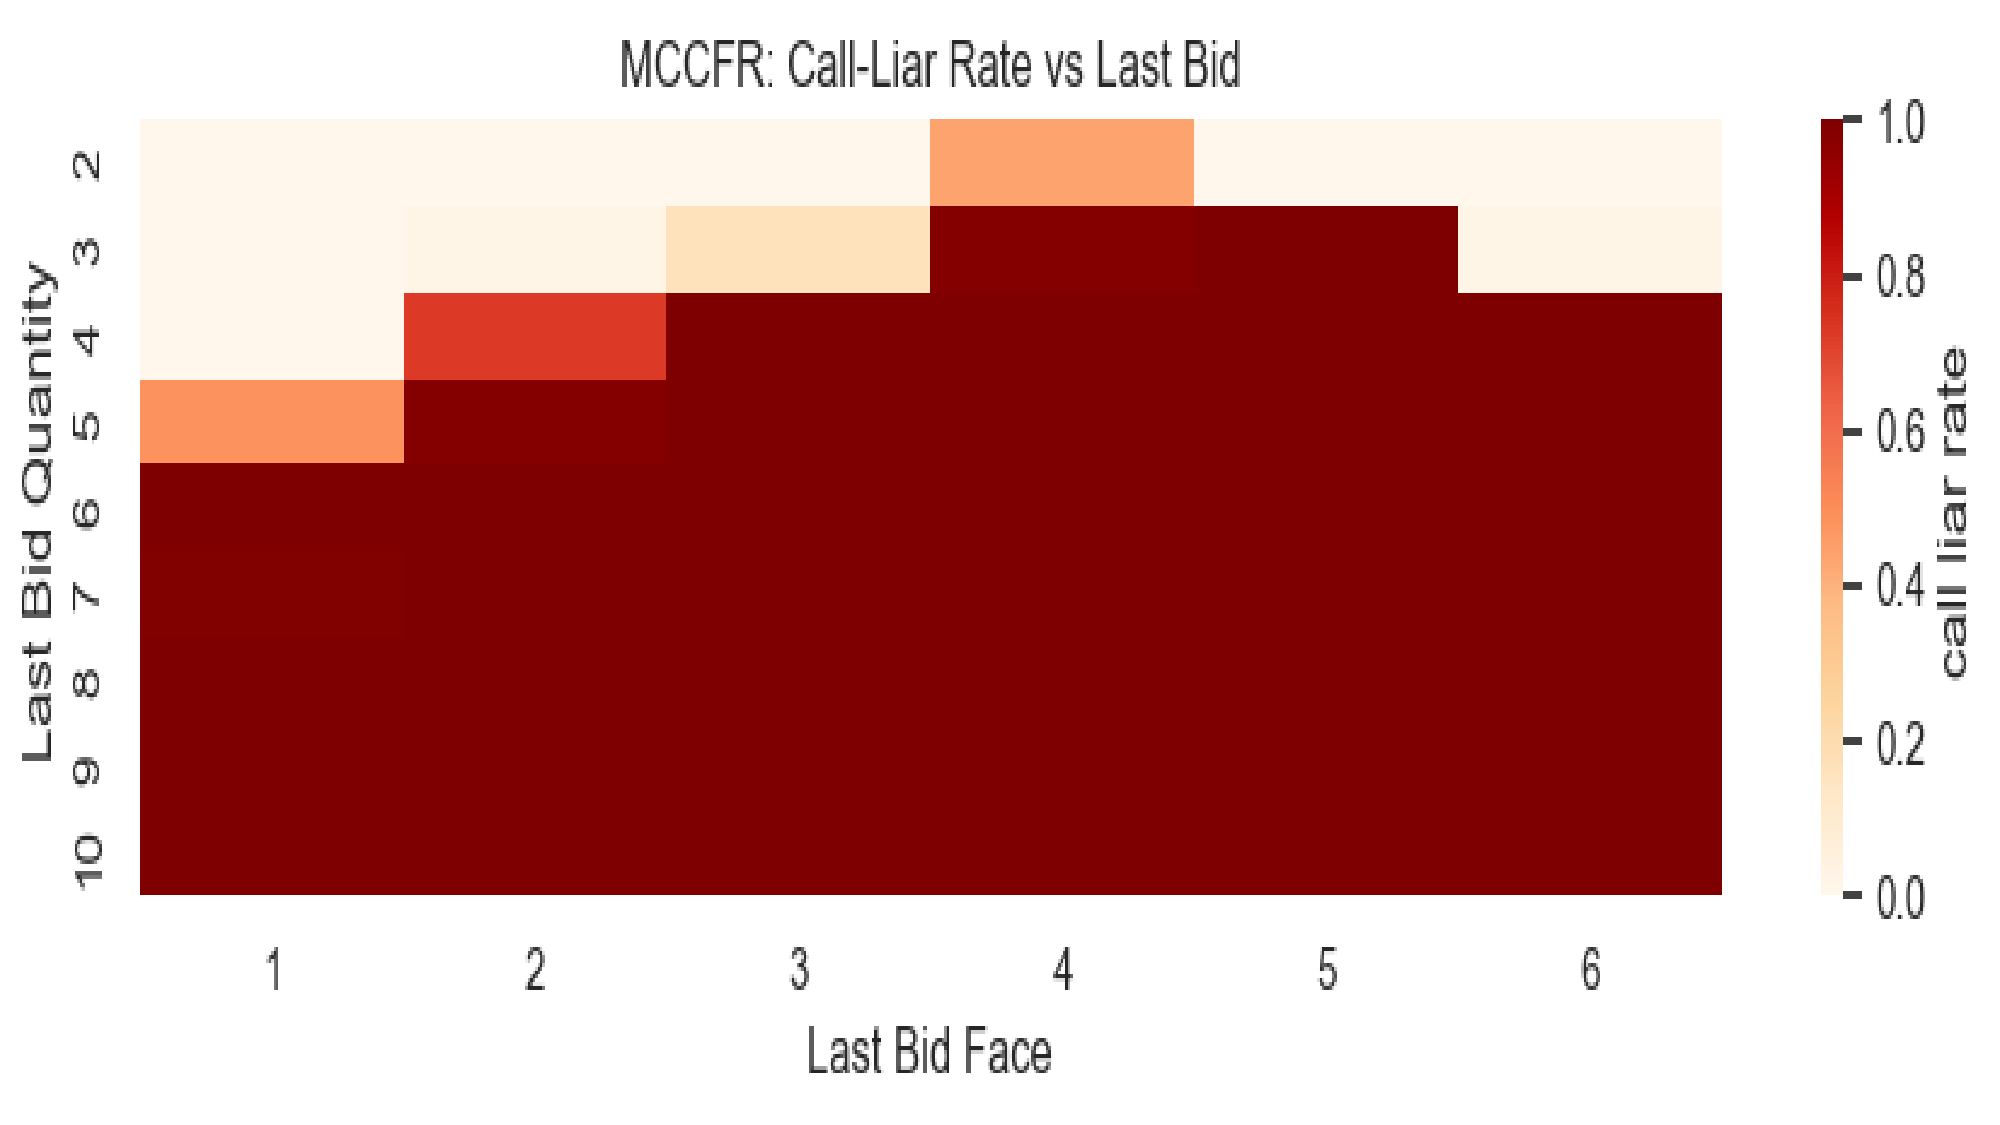
\includegraphics[width=\columnwidth]{images/call_liar_mccfr.pdf}
    \caption{MCCFR call-liar rate as a function of the opponent's last bid quantity and face.}
    \label{fig:app_mccfr_call_liar}
\end{figure}

\begin{figure}[t]
    \centering
    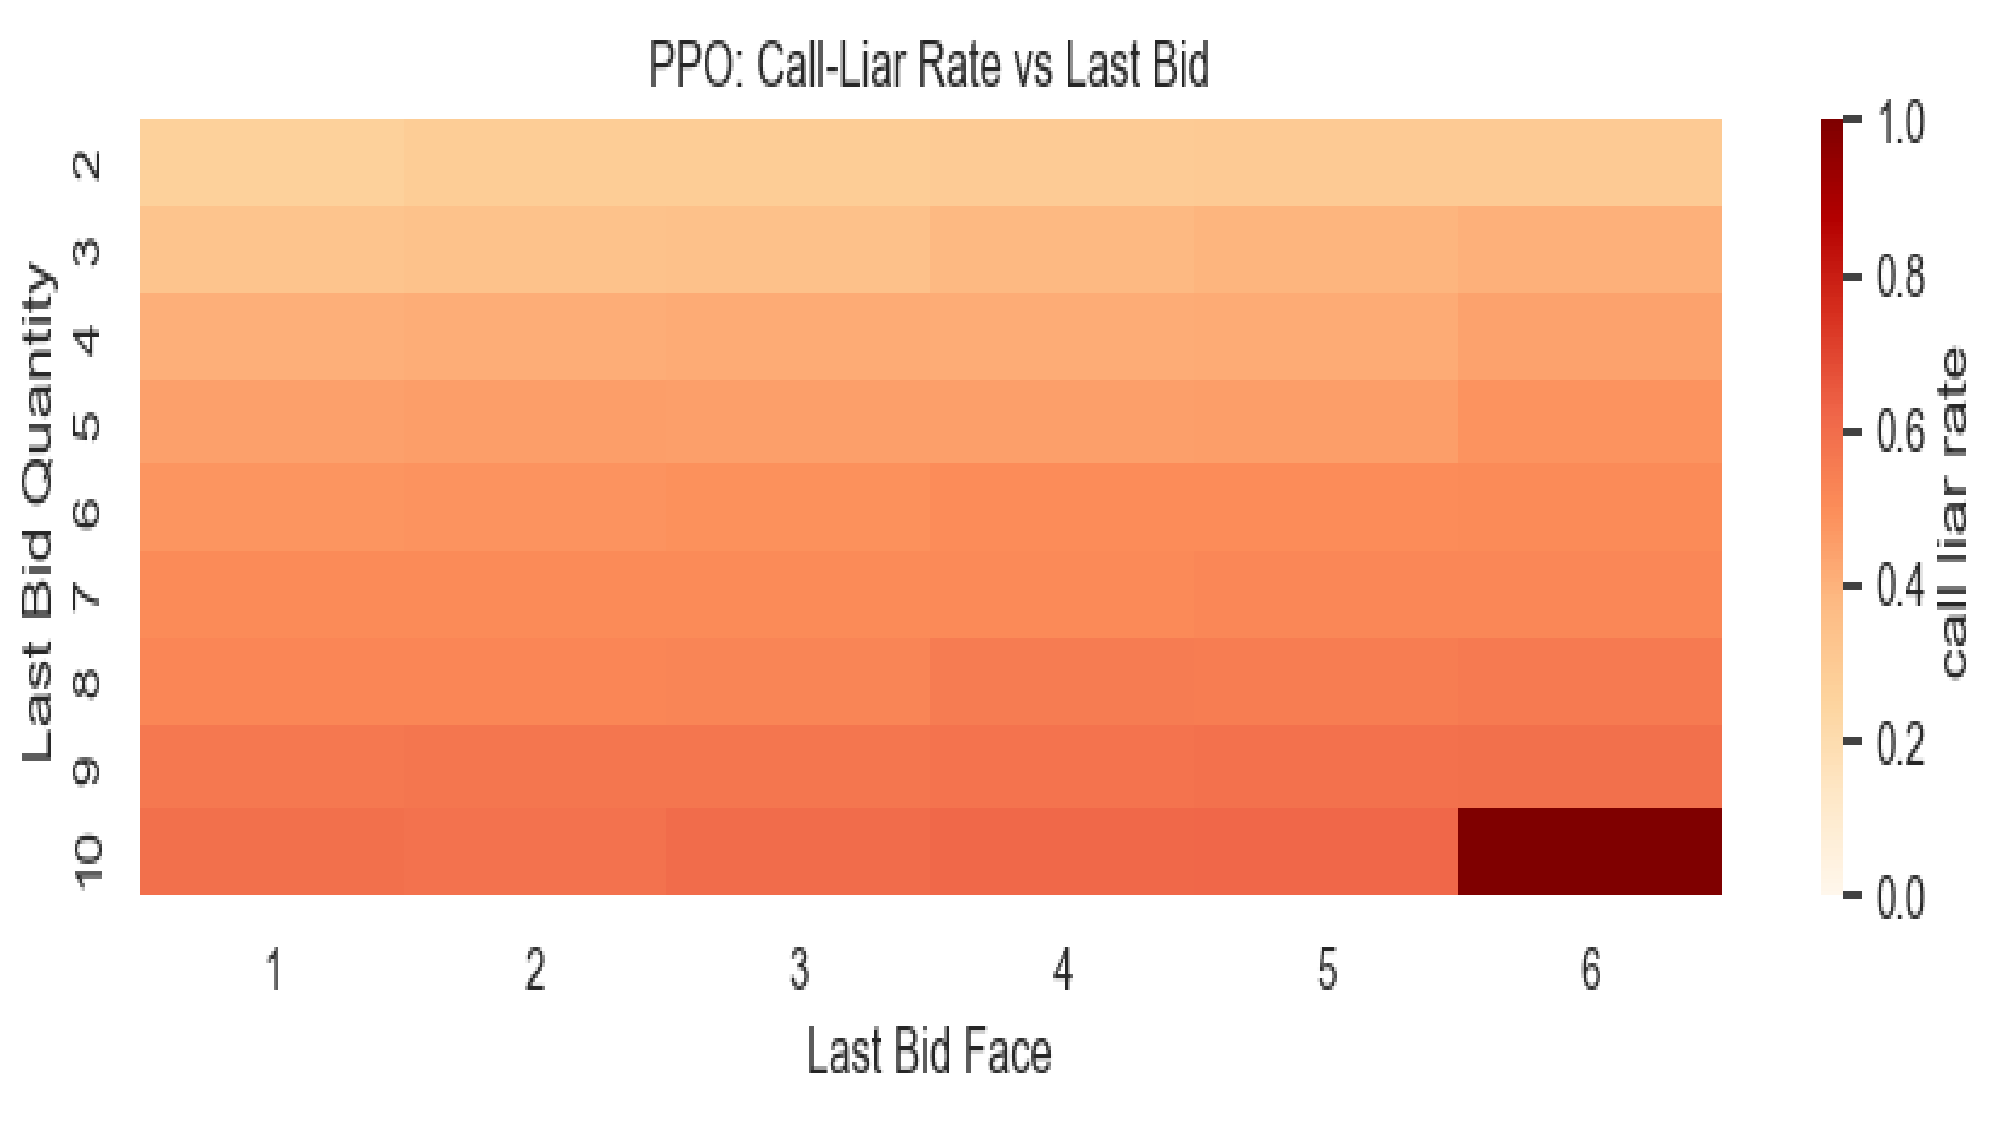
\includegraphics[width=\columnwidth]{images/call_liar_ppo.pdf}
    \caption{PPO call-liar rate as a function of the opponent's last bid quantity and face.}
    \label{fig:app_ppo_call_liar}
\end{figure}

\begin{figure}[t]
    \centering
    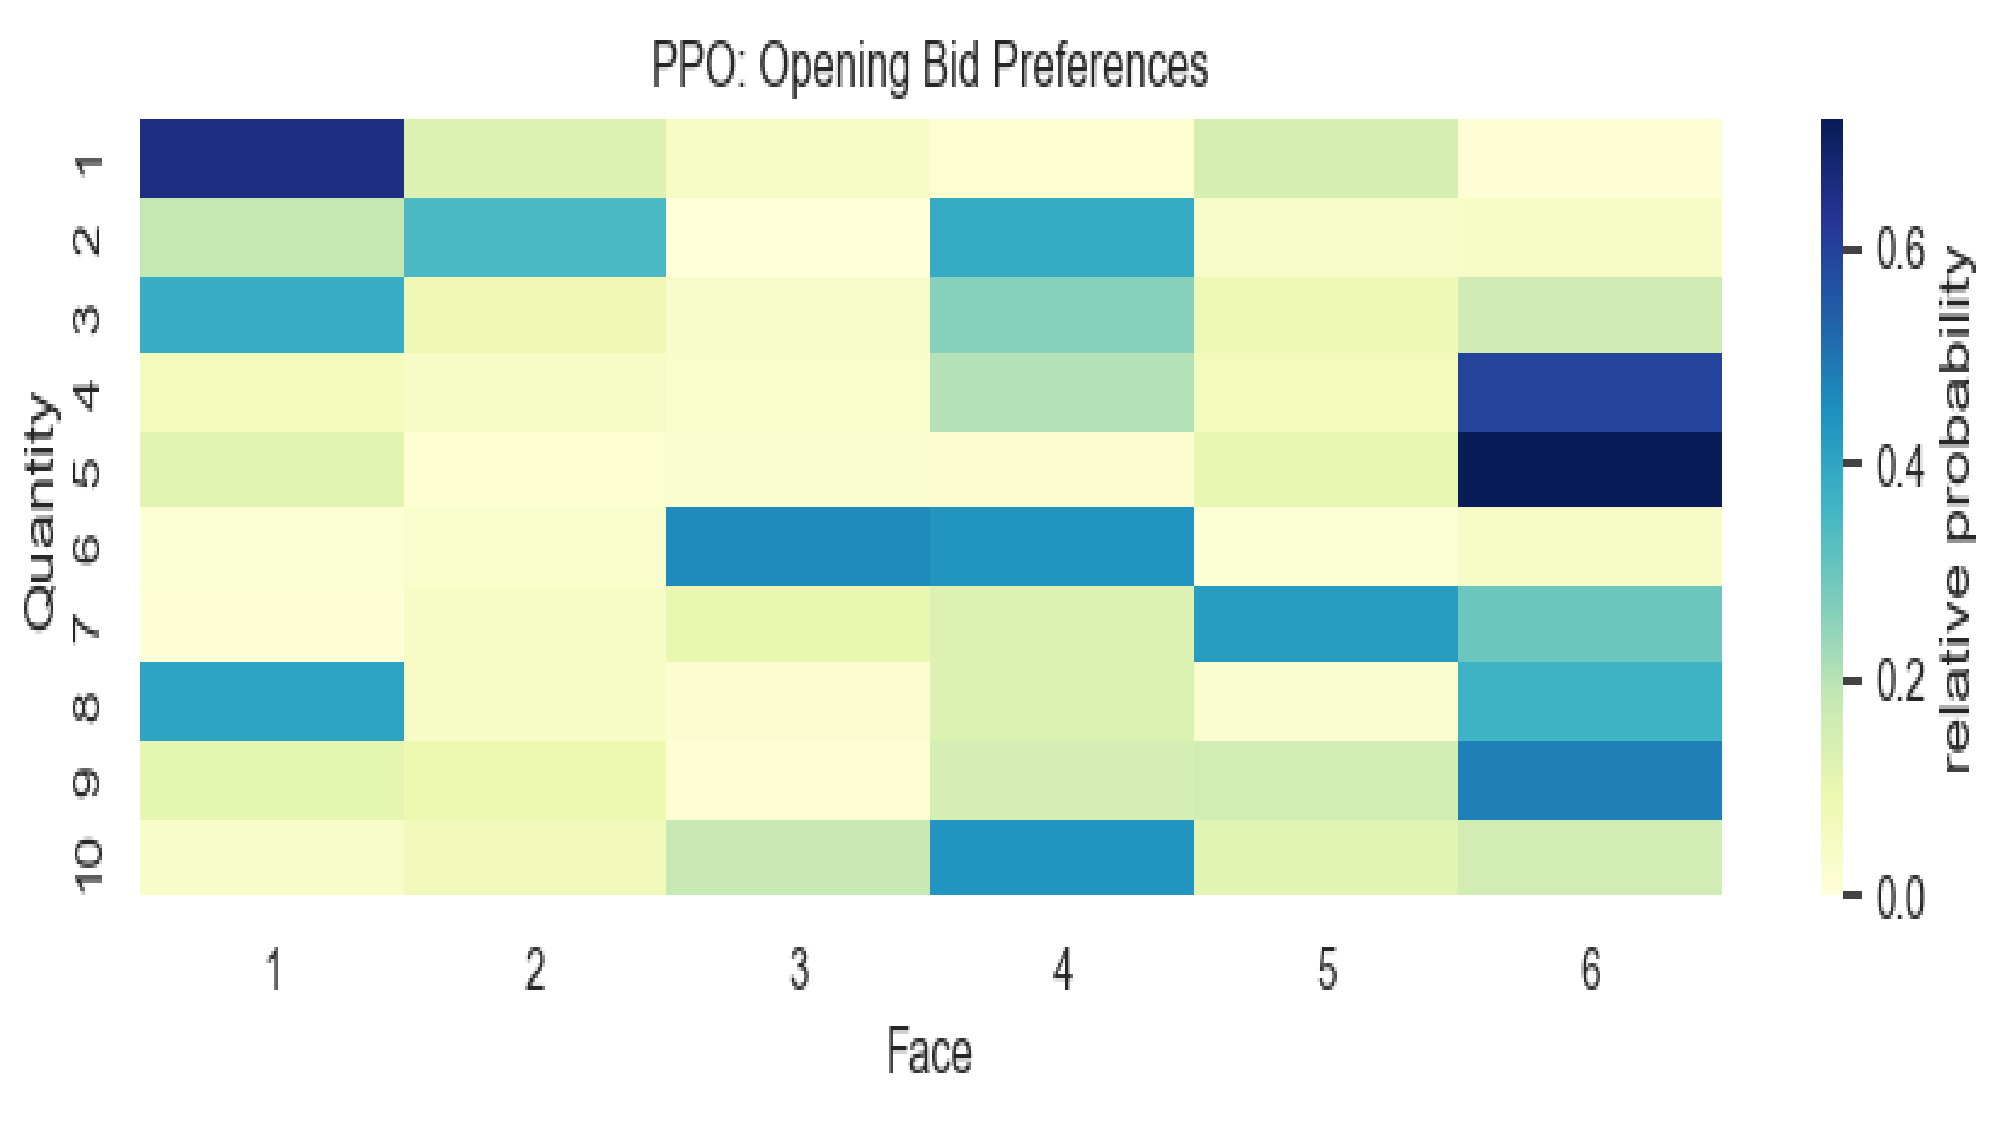
\includegraphics[width=\columnwidth, trim=0cm 4cm 0cm 0cm,clip]{images/opening_bid_preference_ppo.pdf}
    \caption{Opening bid preferences of the PPO agent.}
    \label{fig:app_ppo_opening}
\end{figure}

\begin{figure}[t]
    \centering
    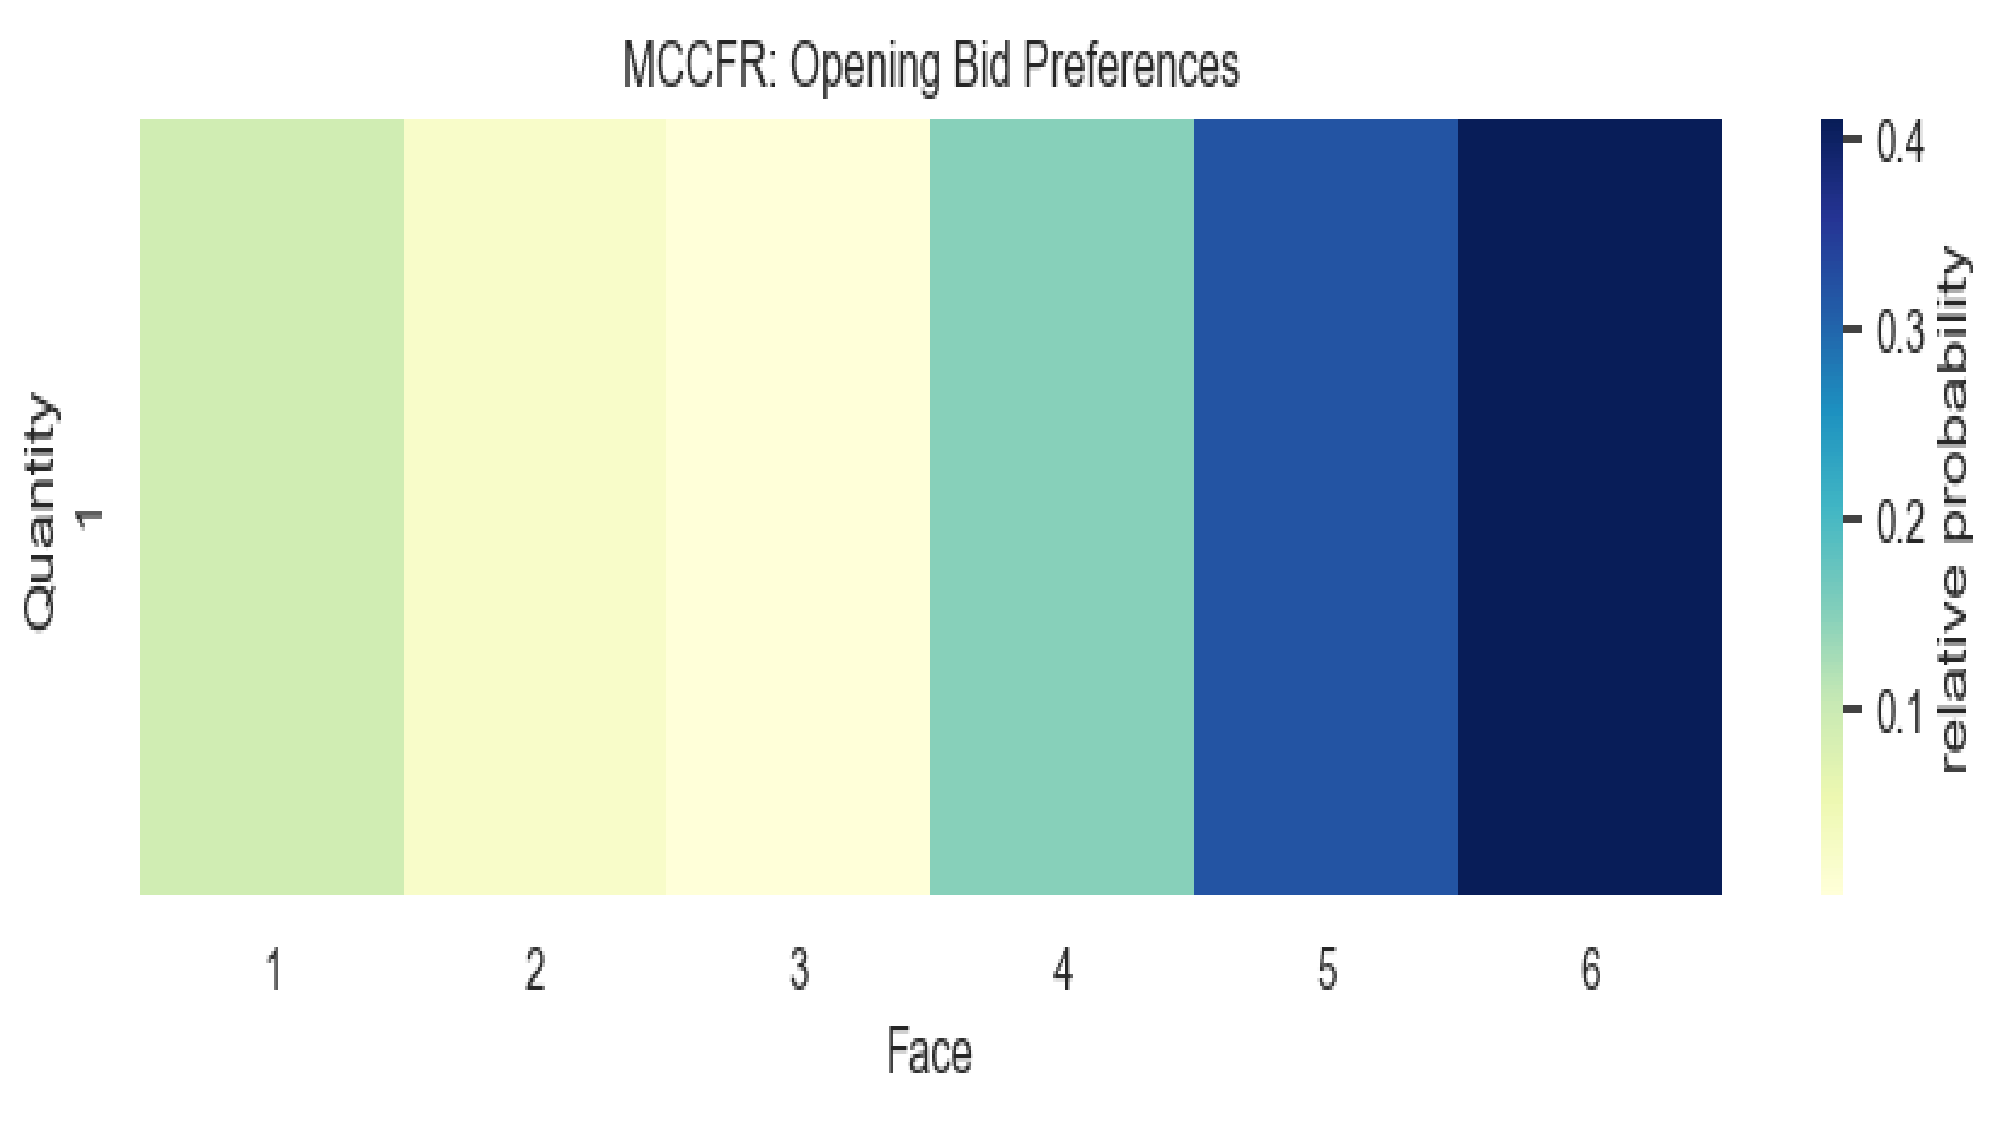
\includegraphics[width=\columnwidth, trim=0cm 4cm 0cm 0cm,clip]{images/opening_bid_preference_mccfr.pdf}
    \caption{Opening bid preferences of the MCCFR agent.}
    \label{fig:app_mccfr_opening}
\end{figure}

\paragraph{Full non-adaptive tournament table.}
Table~\ref{tab:app_agent_behavior_statistics} reports the full static-agent tournament table that was condensed in the main paper.

\begin{table}[t]
\centering
\scriptsize
\resizebox{\columnwidth}{!}{%
\begin{tabular}{lccccc}
\toprule
Agent & Win \% & Avg. steps & Avg. bids & Avg. calls & Avg. bluffs \\
\midrule
\textbf{RL (PPO)} & \textbf{93.14\%} & 19.95 & 13.85 & 6.10 & 5.73 \\
Bayesian & 92.36\% & 22.41 & 16.81 & 5.59 & 4.10 \\
ProbabilityMinRaise & 81.93\% & 36.34 & 30.25 & 6.10 & 4.69 \\
ThresholdLiar & 71.31\% & 47.09 & 41.50 & 5.59 & 4.95 \\
MaxCount & 69.17\% & 26.04 & 20.38 & 5.65 & 4.75 \\
Parity & 67.88\% & 29.05 & 22.58 & 6.47 & 4.24 \\
RandomThreshold & 65.70\% & 45.88 & 40.39 & 5.49 & 4.86 \\
Conservative & 62.71\% & 46.44 & 40.99 & 5.45 & 4.88 \\
CycleFace & 62.42\% & 50.38 & 44.77 & 5.60 & 5.01 \\
Alternator & 62.31\% & 22.16 & 15.16 & 7.00 & 3.81 \\
MinRaise & 62.02\% & 46.47 & 41.02 & 5.45 & 4.85 \\
Mirror & 56.54\% & 30.52 & 24.75 & 5.77 & 5.15 \\
Bluffing & 54.52\% & 40.56 & 34.89 & 5.66 & 4.82 \\
OnesAreWild & 49.98\% & 38.33 & 32.74 & 5.59 & 4.69 \\
SafeFace & 49.82\% & 38.36 & 32.77 & 5.59 & 4.70 \\
NashCFR & 45.42\% & 37.61 & 31.68 & 5.93 & 5.16 \\
RandomFace & 29.48\% & 20.34 & 14.81 & 5.53 & 5.23 \\
ProbabilityMaxRaise & 24.77\% & 16.61 & 11.04 & 5.57 & 5.05 \\
Chaotic & 21.71\% & 18.93 & 12.79 & 6.14 & 4.68 \\
ChaoticSafe & 21.61\% & 18.94 & 12.79 & 6.15 & 4.69 \\
Aggressive & 17.53\% & 16.07 & 10.72 & 5.35 & 5.31 \\
MaxRaise & 17.26\% & 16.40 & 11.06 & 5.35 & 5.15 \\
ChaoticUnsafe & 13.22\% & 19.34 & 13.21 & 6.12 & 4.66 \\
\bottomrule
\end{tabular}}
\caption{Overall win rates in the non-adaptive agent-versus-agent tournament with high-level behavioral statistics.}
\label{tab:app_agent_behavior_statistics}
\end{table}

\begin{figure*}[t]
    \centering
    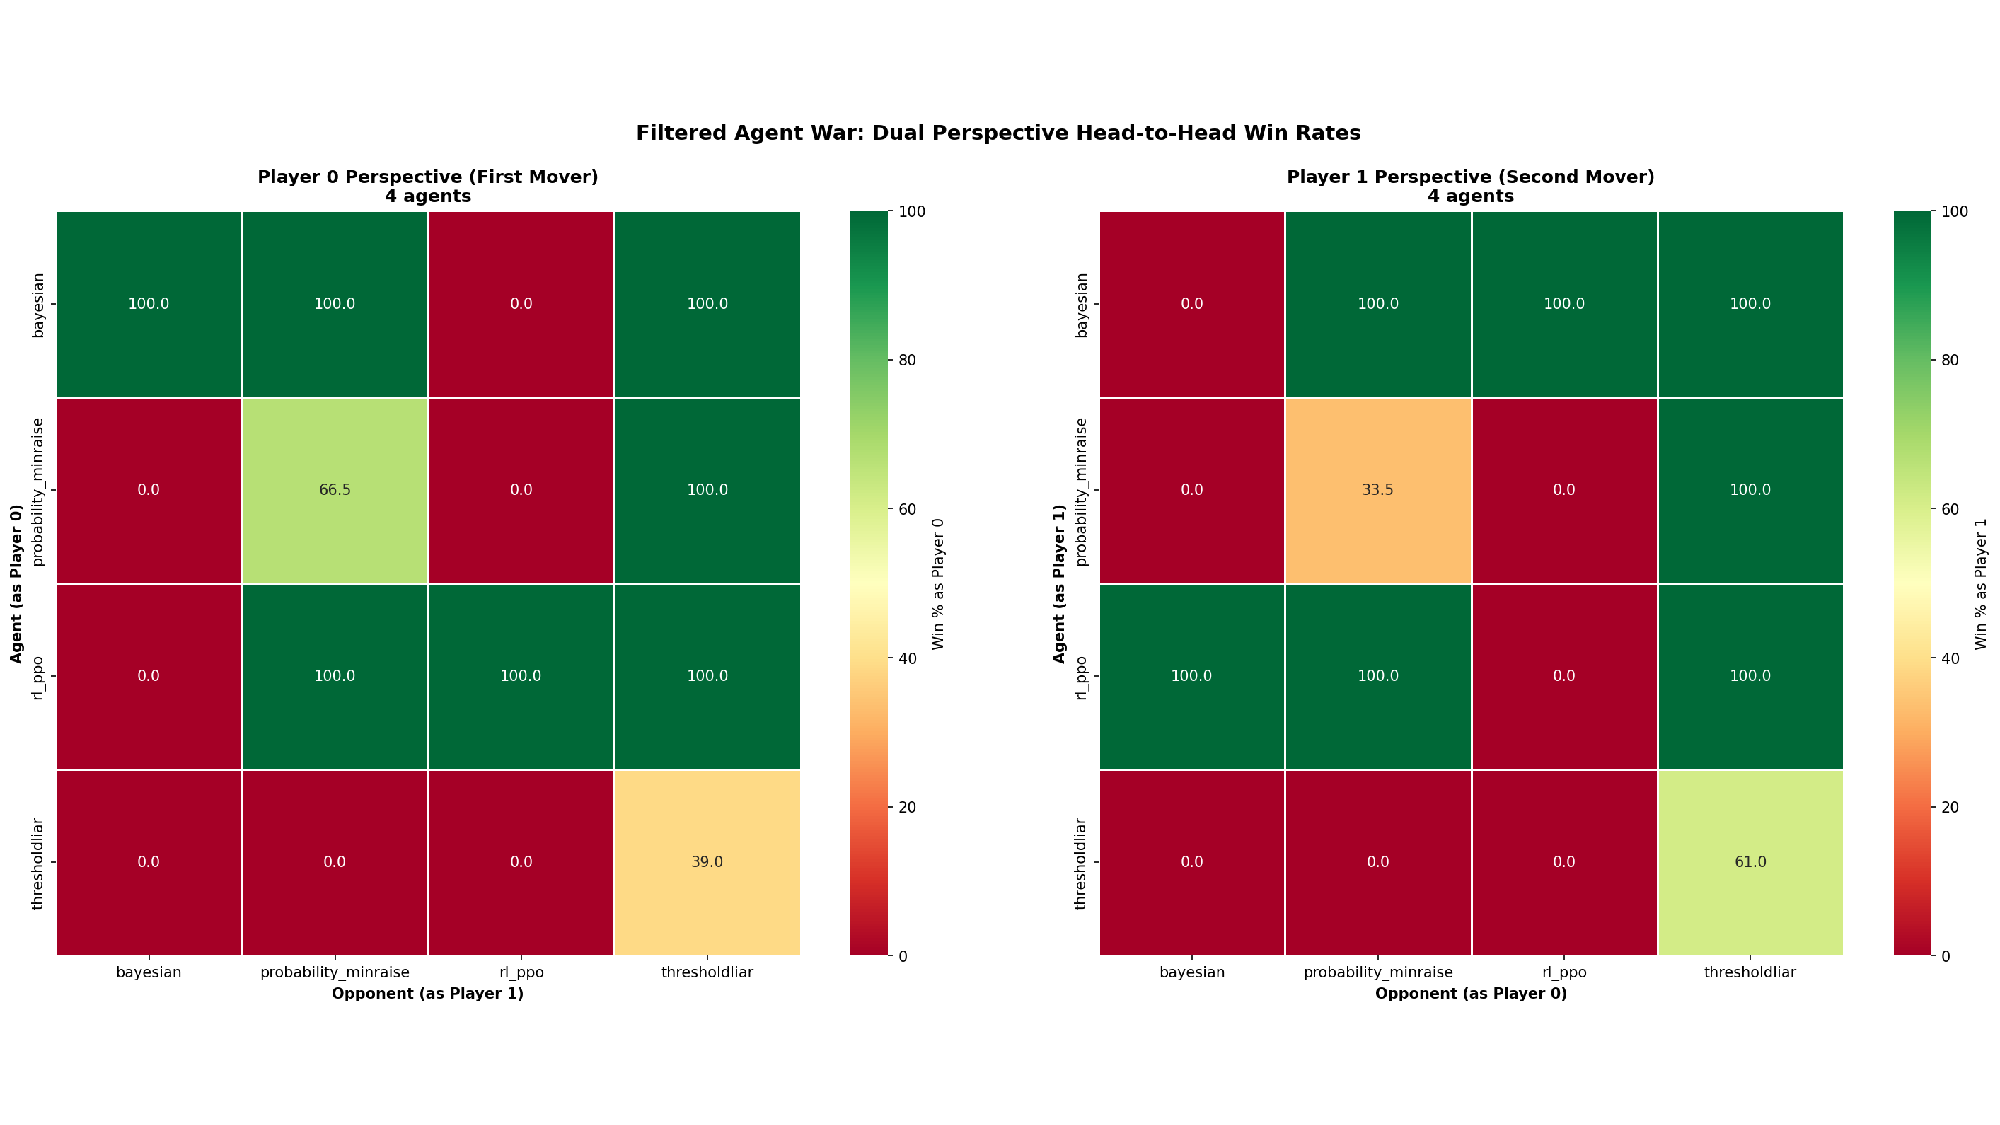
\includegraphics[width=\textwidth, trim=0cm 2cm 0cm 0cm,clip]{images/head_to_head_top_4.pdf}
    \caption{Dual-perspective head-to-head win rates for the top-performing agents. Each cell reports win rates when the row agent plays as Player~0 (first mover, left) or Player~1 (second mover, right).}
    \label{fig:app_head_to_head_top_4}
\end{figure*}

\paragraph{Adaptive-agent identification and per-opponent performance.}
Tables~\ref{tab:app_adaptive_identification} and~\ref{tab:app_adaptive_winrates} provide detailed adaptive-agent results by opponent type.

\begin{table}[t]
\centering
\scriptsize
\begin{tabular}{lcc}
\toprule
Opponent & Accuracy & Mean steps to ID \\
\midrule
AggressiveAgent & 100.0\% & $3.10 \pm 0.94$ \\
BayesianAgent & 100.0\% & $2.00 \pm 0.00$ \\
MaxRaiseAgent & 100.0\% & $3.00 \pm 1.00$ \\
RandomFaceAgent & 93.0\% & $3.00 \pm 1.00$ \\
NashCFRAgent & 92.5\% & $2.00 \pm 0.00$ \\
MirrorAgent & 72.0\% & $3.39 \pm 0.92$ \\
BluffingAgent & 69.5\% & $2.98 \pm 1.00$ \\
MaxCountBidAgent & 50.0\% & $2.00 \pm 0.00$ \\
GeneralistPPO & 50.0\% & $3.00 \pm 0.00$ \\
SafeFaceAgent & 50.0\% & $4.00 \pm 0.00$ \\
ConservativeAgent & 50.0\% & $2.00 \pm 0.00$ \\
CycleFaceAgent & 50.0\% & $2.00 \pm 0.00$ \\
RandomThresholdAgent & 46.5\% & $3.89 \pm 0.45$ \\
ChaoticSafeAgent & 39.0\% & $3.00 \pm 0.88$ \\
ChaoticUnsafeAgent & 36.0\% & $3.03 \pm 0.73$ \\
AlternatorAgent & 26.5\% & $2.00 \pm 0.00$ \\
ChaoticAgent & 19.0\% & $2.95 \pm 0.79$ \\
ThresholdLiarAgent & 18.5\% & $2.00 \pm 0.00$ \\
ProbabilityMinRaiseAgent & 18.0\% & $2.00 \pm 0.00$ \\
MinRaiseAgent & 10.5\% & $2.00 \pm 0.00$ \\
ProbabilityMaxRaiseAgent & 1.5\% & $2.00 \pm 0.00$ \\
\midrule
OnesAreWildAgent & 0.0\% & -- \\
ParityAgent & 0.0\% & -- \\
\bottomrule
\end{tabular}
\caption{Opponent identification accuracy and mean number of steps to correct identification, reported for games in which identification was correct.}
\label{tab:app_adaptive_identification}
\end{table}

\begin{table}[t]
\centering
\scriptsize
\resizebox{\columnwidth}{!}{%
\begin{tabular}{lccc}
\toprule
Opponent & Win \% & $WR_{P0}$ & $WR_{P1}$ \\
\midrule
AggressiveAgent & 100\% & 100\% & 100\% \\
BluffingAgent & 100\% & 100\% & 100\% \\
BayesianAgent & 100\% & 100\% & 100\% \\
FaceFixedRandomAgent & 100\% & 100\% & 100\% \\
CautiousRandomAgent & 100\% & 100\% & 100\% \\
FaceRandomRandomAgent & 100\% & 100\% & 100\% \\
ConservativeAgent & 100\% & 100\% & 100\% \\
CycleFaceAgent & 100\% & 100\% & 100\% \\
MinRaiseAgent & 100\% & 100\% & 100\% \\
MaxRaiseAgent & 100\% & 100\% & 100\% \\
MaxCountBidAgent & 100\% & 100\% & 100\% \\
GeneralistPPO & 100\% & 100\% & 100\% \\
ParityAgent & 100\% & 100\% & 100\% \\
RandomAgent & 100\% & 100\% & 100\% \\
RandomThresholdAgent & 100\% & 100\% & 100\% \\
RandomFaceAgent & 100\% & 100\% & 100\% \\
SafeFaceAgent & 100\% & 100\% & 100\% \\
MirrorAgent & 100\% & 100\% & 100\% \\
NashCFRAgent & 100\% & 100\% & 100\% \\
OnesAreWildAgent & 100\% & 100\% & 100\% \\
ThresholdLiarAgent & 100\% & 100\% & 100\% \\
\midrule
ChaoticAgent & 99\% & 100\% & 99\% \\
ChaoticUnsafeAgent & 99\% & 99\% & 100\% \\
AggressiveRandomAgent & 99\% & 98\% & 100\% \\
ChaoticSafeAgent & 99\% & 100\% & 98\% \\
ProbabilityMaxRaiseAgent & 96\% & 92\% & 100\% \\
ProbabilityMinRaiseAgent & 90\% & 80\% & 100\% \\
AlternatorAgent & 53\% & 48\% & 58\% \\
\bottomrule
\end{tabular}}
\caption{Win rates of the adaptive agent against each opponent, overall and by player position (P0: first mover, P1: second mover).}
\label{tab:app_adaptive_winrates}
\end{table}

\paragraph{Additional diagnostics.}
Tables~\ref{tab:app_latency_analysis}--\ref{tab:app_multi_agent_results} preserve the latency, correlation, and multi-agent transfer diagnostics omitted from the compact main paper.

\begin{table}[t]
\centering
\scriptsize
\begin{tabular}{lc}
\toprule
Agent & Time per turn (ms) \\
\midrule
Bayesian & $0.014 \pm 0.012$ \\
Conservative & $0.005 \pm 0.004$ \\
Nash (CFR) & $0.008 \pm 0.011$ \\
RL (PPO) & $0.570 \pm 1.971$ \\
Adaptive Agent & $0.741 \pm 0.843$ \\
\bottomrule
\end{tabular}
\caption{Agent decision time per turn, reported as mean $\pm$ standard deviation.}
\label{tab:app_latency_analysis}
\end{table}

\begin{table}[t]
\centering
\scriptsize
\resizebox{\columnwidth}{!}{%
\begin{tabular}{lccccc}
\toprule
 & Win \% & Avg. steps & Avg. bids & Avg. calls & Avg. bluffs \\
\midrule
Win \%        & - & 0.48 & 0.47 & 0.17 & 0.12 \\
Avg. steps   & - & - & 0.999 & 0.26 & 0.01 \\
Avg. bids    & - & - & - & 0.29 & 0.03 \\
Avg. calls   & - & - & - & - & 0.51 \\
Avg. bluffs  & - & - & - & - & - \\
\bottomrule
\end{tabular}}
\caption{Pearson correlation matrix between win rate and behavioral statistics.}
\label{tab:app_correlation_matrix}
\end{table}

\begin{table}[t]
\scriptsize
\centering
\begin{tabular}{llccc}
\toprule
Game setting & Agent & Wins & Win\% & Avg turns \\
\midrule
\multirow{3}{*}{3 agents (heuristics)}
 & \textbf{Bayesian} & \textbf{991} & \textbf{99.1} & 30.0 \\
 & Conservative & 9 & 0.9 & 24.7 \\
 & Probability MaxRaise & 0 & 0.0 & 9.3 \\
\midrule
\multirow{3}{*}{3 agents (with PPO)}
 & \textbf{Bayesian} & \textbf{947} & \textbf{94.7} & 24.9 \\
 & Conservative & 50 & 5.0 & 20.9 \\
 & RL (PPO) & 3 & 0.3 & 13.6 \\
\midrule
\multirow{4}{*}{4 agents}
 & \textbf{Bayesian} & \textbf{887} & \textbf{88.7} & 24.2 \\
 & Conservative & 94 & 9.4 & 21.5 \\
 & Probability MaxRaise & 0 & 0.0 & 10.5 \\
 & RL (PPO) & 19 & 1.9 & 20.0 \\
\bottomrule
\end{tabular}
\caption{Results of 1{,}000 multi-agent Liar's Dice games across different agent configurations.}
\label{tab:app_multi_agent_results}
\end{table}




\end{document}
